\section{Demand Controlled Ventilation }\label{demand-controlled-ventilation}

ASHRAE Standard 62.1, Ventilation for Acceptable Indoor Air Quality, contains provisions that allow building ventilation systems to vary the amount of outdoor ventilation air delivered to occupied zones based on feedback from sensors that monitor various indoor air contaminants (ASHRAE 2007). Although not a contaminant of concern in most buildings, carbon dioxide (CO\(_{2}\)) levels can be monitored as an indicator of building occupancy and the associated human bioeffluent concentration. Demand controlled ventilation (DCV) is being increasingly used to modulate outdoor ventilation air based on real-time occupancy (Emmerich and Persily 1997, Schell et al. 1998, Schell and Int-Hout 2001). Modulating the outdoor ventilation air while maintaining proper indoor air quality has the potential for large energy savings compared to constant rate ventilation systems that are typically designed to provide outdoor ventilation air based on maximum anticipated occupancy.

EnergyPlus can model DCV by the ventilation rate procedure (VRP) defined in ASHRAE Standard 62.1-2007/2010 for single and multiple path systems, and the indoor air quality procedure (IAQP) defined in Standard 62. The VRP first calculates the breathing-zone outdoor air flow rate based on two components -- the zone occupant component and the zone floor area component, then it calculates the zone supply outdoor air flow rate considering the zone air distribution effectiveness and secondary recirculation (for mult-path systems only), and finally calculates the system outdoor air flow rate considering the zone diversity and system ventilation efficiency. The user must include the following five objects in their input data file in order to model DCV (using VRP or IAQP):

\begin{itemize}
  \item \textbf{AirLoopHVAC:OutdoorAirSystem} to simulate the mixed air box of the air loop
  \item \textbf{Controller:MechanicalVentilation} with the DCV flag set to `Yes' to determine the minimum outdoor air flow rate to be provided by the mixed air box
  \item \textbf{Controller:OutdoorAir} to control the outside air flow rate introduced via the mixed air box
  \item \textbf{DesignSpecification:OutdoorAir} to describe the outdoor air requirements for each zone
  \item \textbf{DesignSpecification:ZoneAirDistribution} to describe air distribution effectiveness and secondary recirculation (for multi-path ventilation systems) for each zone
\end{itemize}

The outdoor air system (AirLoopHVAC:OutdoorAirSystem) is a subsystem of an AirLoopHVAC which handles the mixed air portion of the primary air system: the system relief air, the outside air inlet, and any components and controllers associated with the system relief air and outside air streams. The inputs for this object are fully described in the EnergyPlus Input Output Reference. Determining the outdoor air ventilation rate and introducing this ventilation via the mixed air box are accomplished by the mechanical ventilation and outdoor air controller objects.

The VRP currently requires outdoor air ventilation rates to be determined based on the floor area of each occupied zone plus the number of people in each zone. The number of people varies based on the setting of the DCV flag in the Controller:MechanicalVentilation object. For using occupancy at every time step, the DCV flag must be set to `Yes'. The outdoor air ventilation rate can then be reset dynamically as operating conditions change (e.g., variations in occupancy). The Controller:MechanicalVentilation object simplifies the procedure for calculating these outdoor air ventilation requirements and resetting them based on varying occupancy levels. This is particularly useful for large air distribution systems that serve a number of different zone types with varying occupancy levels.

The IAQP (ASHRAE 2007) is a design procedure in which outdoor air intake and other system design parameters are based on an analysis of contaminant sources, and contaminant concentration targets. Although carbon dioxide is not considered as an indoor contaminant but is considered as an indicator of indoor air quality in buildings, EnergyPlus uses IAQP to control carbon dioxide. In addition, a generic contaminant may be introduced. The current IAQP in EnergyPlus allows credit to be taken for controls that can be reliably demonstrated to result in indoor carbon dioxide and generic contaminant concentrations equal to or lower that those achieved using the VRP. The IAQP may also be used where the design is intended to attain specific target carbon dioxide and generic contaminant levels.

\subsection{Ventilation Rate Procedure}\label{ventilation-rate-procedure}

\subsubsection{Calculation of zone minimum outdoor air flow}\label{calculation-of-zone-minimum-outdoor-air-flow}

For the i-th zone, first the breathing-zone outdoor air flow is calculated:

\begin{equation}
{V_{bz,i}} = {R_{p,i}} \times {P_i} + {R_{a,i}} \times {A_i} \times {SchedFrac_i}
\end{equation}

where:

\({V_{bz,i}}\) is the breathing-zone outdoor air flow (m\(^3\)/s)

\({R_{p,i}}\) is the ventilation rate per person (m\(^3\)/s-person)

\({P_i}\) is the number of occupants for the zone

\({R_{a,i}}\) is the ventilation rate per floor area (m\(^3\)/s-m\(^2\))

\({A_i}\) is the floor area of the zone (m\(^2\))

\({SchedFrac_i}\) is the Outdoor Air Schedule value for the zone, if specified in the corresponding DesignSpecification:OutdoorAir object (defaults to 1.0)

\(i\) is the index of the zone or zone list.

Next, the i-th zone outdoor air flow is calculated:

\begin{equation}
{V_{oz,i}} = {V_{bz,i}}/{E_i}
\end{equation}

Where:

\({V_{oz,i}}\) is the zone outdoor air flow (m\(^3\)/s)

\({E_i}\) is the zone air distribution effectiveness, see following figure for ASHRAE recommended values.

\begin{figure}[hbtp] % fig 195
\centering
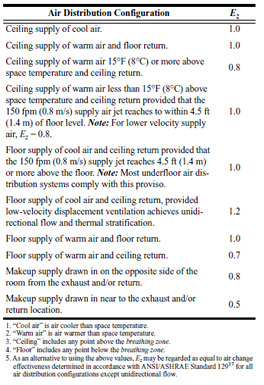
\includegraphics[width=0.9\textwidth, height=0.9\textheight, keepaspectratio=true]{media/image4716.png}
\caption{Zone Air Distribution Effectiveness Typical Values (Source: ASHRAE Standard 62.1-2010) \protect \label{fig:zone-air-distribution-effectiveness-typical}}
\end{figure}

\subsubsection{Calculation of system minimum outdoor air flow}\label{calculation-of-system-minimum-outdoor-air-flow}

Occupant diversity, \emph{D}, is the expected peak system population, \emph{Ps}, divided by the sum of the design zone population for all the zones attached to the air system, \emph{Pzsum}. In EnergyPlus, \emph{D}, \emph{Ps}, and \emph{Pzsum} are determined by a side calculation, in the routine DetermineSystemPopulationDiversity.  This routine loops over each airloop in the model and processes the People descriptions in each zone attached to a given airloop.  The design level is summed and includes zone multipliers.  The concurrent system peak population is calculated by stepping through a full year of zone timesteps and multiplying the people schedules (input field Number of People Schedule Name) to the design level and summing up a total people concurrent at each timestep.  The largest value for the total concurrent people on a system is used for \emph{Pzsum}.  For single zone air systems, \emph{D} is forced to be 1.0 because there is no diversity that could come from serving multiple zones. 

For single zone systems, the system outdoor air flow:

\begin{equation}
{V_{ot}} = {V_{oz}}
\end{equation}

For 100\% outdoor air multi-zone systems, the system outdoor air flow:

\begin{equation}
{V_{ot}} = \mathop \sum \limits_{i = 1}^{allzones} {V_{oz,i}}
\end{equation}

For non 100\% outdoor air multi-zone systems, the system outdoor air flow:

\begin{equation}
{V_{ot}} = {V_{ou}}/{E_v}
\end{equation}

where:

\({V_{ou}}\) is the uncorrected system outdoor air flow (m\(^3\)/s)

\begin{equation}
{V_{ou}} = \mathop \sum \limits_{i = 1}^{allzones} ({R_{p,i}} \times {P_i} \times {SchedFrac_i}) + \mathop \sum \limits_{i = 1}^{allzones} ({R_{a,i}} \times {A_i} \times {SchedFrac_i})
\end{equation}

\({X_s}\) is the uncorrected system outdoor air fraction

\begin{equation}
{X_s} = {V_{ou}}/{V_{ps}}
\end{equation}

\({V_{ps}}\) is the system supply air flow (m\(^3\)/s)

\({Z_{d,i}}\) is the zone outdoor air fraction

\begin{equation}
{Z_{d,i}} = {V_{oz,i}}/{V_{dz,i}}
\end{equation}

\({V_{dz,i}}\) is the zone supply air flow (m\(^3\)/s)

\({E_v}\) is the system ventilation efficiency, determined as the minimum of the zone ventilation efficiency among all ventilation zones served by the air handler

\emph{Ev} is the minimum of (\emph{Evz})

\emph{Evz} is the zone ventilation efficiency, determined differently for single-path and multi-path systems.

\textbf{\emph{For single-path systems:}}

\begin{equation}
Evz = 1 + Xs - Z_{d,i}
\end{equation}

\textbf{\emph{For multi-path systems:}}

\begin{equation}
Evz = (Fa + Xs·Fb - Z_{d,i}·Ep·Fc)/Fa
\end{equation}

where system air fractions \emph{Fa}, \emph{Fb}, and \emph{Fc} are determined as follows:

\begin{equation}
Fa = Ep + {(1 - Ep) · Er}
\end{equation}

\begin{equation}
Fb = Ep
\end{equation}

\begin{equation}
Fc = 1 - (1 - Ez) · (1 - Er) · (1 - Ep)
\end{equation}

where:

\emph{Ep} is the zone primary air fraction. For dual-fan dual-duct systems, the zone primary air is the air from the cold duct.  This can be expressed as: \emph{Ep = Vpz/Vdz,i}

\emph{Er} is the zone secondary recirculation fraction.

Single-path systems are special cases of multi-path systems where \emph{Er} = 0, \emph{Ep} = 1, \emph{Fa} = \emph{Fb =} \emph{Fc} = 1.0

The zone secondary recirculation fraction Er is determined by the designer based on system configuration. For plenum return systems with secondary recirculation (e.g., fan-powered VAV with plenum return) Er is usually less than 1.0, although values may range from 0.1 to 1.2 depending upon the location of the ventilation zone relative to other zones and the air handler. For ducted return systems with secondary recirculation (e.g., fan-powered VAV with ducted return), Er is typically 0.0, while for those with system-level recirculation (e.g, dual-fan dual-duct systems with ducted return) Er is typically 1.0. For other system types, Er is typically 0.75.

The program then calculates the minimum outdoor air flow fraction based on the information provided in the object Controller:MechanicalVentilation and the maximum branch air flow rate as follows:

\begin{equation}
MechVentOutsideAirMinFrac = {V_{ot}} {\rho_{std}} / {\dot m_{maxbranch}}
\end{equation}

where MechVentOutsideAirMinFrac is the outdoor air minimum fraction based on all zones specified in the Controller:MechanicalVentilation object.

Controller:OutdoorAir controls the amount of outdoor ventilation air introduced via the mixed air box based on several user inputs. The user can define the minimum outdoor air flow rate as a percentage of the system's supply air flow rate (e.g., for a variable-air volume system) or a fixed minimum outdoor air flow rate (not as a percentage but a fixed value) (field MinimumLimit). DCV, using the Controller:MechanicalVentilation object in conjunction with the Controller:OutdoorAir object, allows a third option for setting the minimum outdoor air flow. Economizer operation can also be specified to increase the outdoor air flow above the minimum flow rate to provide free cooling when conditions permit (Controller:OutdoorAir, field Economizer Control Type).

EnergyPlus uses the \emph{largest} outdoor air flow rate calculated by the various methods described above when modeling system performance (as long this rate doesn't exceed the maximum flow rate specified for the main air loop branch or for the outdoor air controller itself).

The method used to calculate the outdoor ventilation air flow rate for each system simulation time step is described in more detail below. The figure below schematically illustrates air flow paths used in the calculation of outdoor air flow rate.

\begin{figure}[hbtp] % fig 196
\centering

\includegraphics[width=0.9\textwidth, height=0.9\textheight, keepaspectratio=true]{media/image4731.png}
\caption{Demand Control Ventilation -- Air Flow Paths \protect \label{fig:demand-control-ventilation-air-flow-paths}}
\end{figure}

The minimum outdoor air flow rate is first calculated based on the minimum outdoor air flow rate and the minimum outdoor air schedule value as defined by the user inputs for the object Controller:OutdoorAir:

\begin{equation}
\dot{m}_{minOA} = \dot{V}_{minOA} \cdot MinOAScheduleValue \cdot {\rho_{std}}
\end{equation}

where:

\({\dot{m}_{minOA}}\) is the minimum outdoor air flow rate for this time step (kg/s)

\({\dot{V}_{minOA}}\) is the minimum outdoor air flow rate defined in Controller:OutdoorAir (m\(^{3}\)/s)

\emph{MinOAScheduleValue} is the minimum outdoor air schedule value defined by the schedule identified in Controller:OutdoorAir

\({\rho_{std}}\) is the standard air density (1.204 kg/m\(^{3}\)) adjusted for the local barometric pressure (standard barometric pressure corrected for altitude, ASHRAE 1997 HOF pg. 6.1).

The outdoor air minimum fraction is then calculated as the ratio of the minimum outdoor air flow rate calculated above to the maximum air flow rate defined in the Branch statement for the main air loop (converted to mass flow rate).

\begin{equation}
  OutAirMinFrac = \frac{\dot{m}_{minOA}}{\dot{m}_{max,branch}}
\end{equation}

where \({\dot{m}_{minOA}}\) is the maximum branch air volume flow rate times \(\rho_{std}\) (kg/s).

The program then calculates the minimum outdoor air flow fraction (\emph{MechVentOutsideAirMinFrac}) according to the VRP based on the information provided in the object Controller:MechanicalVentilation and the maximum branch air flow rate.

The algorithm then uses the larger of these outdoor air minimum fractions in subsequent calculations, and also makes sure that the resulting fraction is between 0 and 1.

\begin{equation}
OutAirMinFrac = MAX\left( {OutAirMinFrac,MechVentOutsideAirMinFrac} \right)
\end{equation}

\begin{equation}
OutAirMinFrac = MIN\left( {MAX\left( {OutAirMinFrac,0.0} \right),1.0} \right)
\end{equation}

The algorithm goes on to determine if economizer operation is possible based on the user inputs and the current conditions of the outdoor air and return air. If conditions permit economizer operation, the outdoor air flow fraction is increased beyond the minimum fraction to meet the mixed air setpoint temperature (setpoint temperature assigned to the node defined in field ``Control\_Node'' of Controller:OutdoorAir).

\begin{equation}
OAFrac = MAX(OutAirMinFrac,EconomizerOAFrac)
\end{equation}

The mass flow rate of outdoor air is then calculated based on the outdoor air fraction determined above and the mixed (supply) air mass flow rate:

\begin{equation}
{\dot m_{OA}} = OAFrac * {\dot m_{MixedAir}}
\end{equation}

where:

\({\dot m_{OA}}\) is the mass flow rate of outdoor air (kg/s)

\(OAFrac\) is the fraction of outdoor air in the mixed (supply) air stream

\({\dot{m}_{MixedAir}}\) is the mass flow rate of the mixture of return air and outdoor ventilation air (kg/s).

The algorithm checks to make sure the calculated outdoor air mass flow rate is greater than or equal to the air flow rate being exhausted.

\begin{equation}
{\dot m_{OA}} = MAX\left( {{{\dot m}_{OA}},{{\dot m}_{ExhaustAir}}} \right)
\end{equation}

If a fixed minimum outdoor air flow rate is specified (field Minimum Limit Type in Controller:OutdoorAir) for a continuous air flow system, the program makes sure that the outdoor air mass flow rate is greater than or equal to the minimum outdoor air flow rate specified by the user.

\begin{equation}
{\dot m_{OA}} = MAX\left( {{{\dot m}_{OA}},{{\dot m}_{\min OA}}} \right)
\end{equation}

The outdoor air mass flow rate should be less than or equal to the mixed (supply) air flow rate, and the outdoor air flow rate is reset if necessary.

\begin{equation}
{\dot m_{OA}} = MIN\left( {{{\dot m}_{OA}},{{\dot m}_{MixedAir}}} \right)
\end{equation}

The outdoor air mass flow rate should also be less than or equal to the maximum outdoor air flow rate specified by the user, and the outdoor air flow rate is reset if necessary.

\begin{equation}
{\dot m_{OA}} = MIN\left( {{{\dot m}_{OA}},{{\dot m}_{MaxOA}}} \right)
\end{equation}

where \({\dot m_{MaxOA}}\) is the maximum outdoor air mass flow rate which is equal to the maximum outdoor air volume flow rate from Controller:OutdoorAir times \({\rho_{std}}\) (kg/s).

Finally, the relief air flow rate is calculated as the difference between the outside and exhaust air mass flow rates.

\begin{equation}
{\dot m_{ReliefAir}} = MAX\left( {{{\dot m}_{OA}} - {{\dot m}_{ExhaustAir}},0.0} \right)
\end{equation}

\subsection{Indoor Air Quality Procedure}\label{indoor-air-quality-procedure}

Like VRP, the user must include the following three objects in their input data file in order to model CO\(_{2}\)-based DCV with IAQP:

\begin{itemize}
  \item \textbf{AirLoopHVAC:OutdoorAirSystem} to simulate the mixed air box of the air loop
  \item \textbf{Controller:MechanicalVentilation} to determine the minimum outside air flow rate to be provided by the mixed air box
  \item \textbf{Controller:OutdoorAir} to control the outside air flow rate introduced via the mixed air box
\end{itemize}

The outdoor air mass flow rate provided by the air loop is calculated as below:

\begin{equation}
{\dot m_{OA}} = \sum\limits_i^N {{{\dot m}_{OA,z,i}} \times {SchedFrac_i}}
\end{equation}

where:

\({\dot m_{OA,z,i}}\) is the outdoor air mass flow rate for the ith zone as calculated according to section Carbon Dioxide Prediction located elsewhere in this document.

\({SchedFrac_i}\) is the Outdoor Air Schedule value for the zone, if specified in the corresponding DesignSpecification:OutdoorAir object (defaults to 1.0)

N is the number of zones served by the air loop, which is provided in the input for a Controller:MechanicalVentilation object.

\subsection{Proportional Control}\label{proportional-control}

The control has three choices: ProportionalControlBasedonOccupancySchedule,  ProportionalControlBasedonDesignOccupancy, and ProportionalControlBasedOnDesignOARate. The difference is occupancy level in the first two choices. The former uses real time occupancy, while the latter uses design occupancy level. The third choice is used to calculate the outdoor airflow rate based on design outdoor air flow rate, specified in the DesignSpecification:OutdoorAir object. Like Ventilation Rate Procedure and the Indoor Air Quality Procedure, the following three objects must be included in the input data file in order to model CO\(_{2}\)-based DCV with Proportional Control:

\begin{itemize}
  \item \textbf{AirLoopHVAC:OutdoorAirSystem} to simulate the mixed air box of the air loop
  \item \textbf{Controller:MechanicalVentilation} to determine the minimum outside air flow rate to be provided by the mixed air box
  \item \textbf{Controller:OutdoorAir} to control the outside air flow rate introduced via the mixed air box
\end{itemize}

For the i-th zone, the outdoor air mass flow rate provided by the air loop is calculated as below:

\begin{enumerate}
\item The required intake flow of outdoor air for the design zone population, \emph{P\(_{z,i}\)}
\end{enumerate}


\begin{equation}
{V_{ot - design,i}} = \frac{{\left( {{R_{p,i}}.{P_{z,i}} \times {SchedFrac_i}} \right) + ({R_{a,i}}.{A_{z,i}} \times {SchedFrac_i})}}{{{E_i}}}
\end{equation}

If ProportionalControlBasedOnDesignOARate is specified, the required intake flow rate will be revised as:

\begin{equation}
{V_{ot - design,i}} = \frac{Design Outdoor Air Flow Rate_i} {E_i}
\end{equation}

The Design Outdoor Air Flow Rate is determined in the DesignSpecification:OutdoorAir object. 

\begin{enumerate}
\setcounter{enumi}{1}
\item The required intake flow of outdoor air when the zone is unoccupied i.e.~ \emph{P\(_{z,i}\)} = 0
\end{enumerate}

\begin{equation}
{V_{ot - min,i}} = \frac{{({R_{a,i}}.{A_{z,i}} \times {SchedFrac_i})}}{{{E_i}}}
\end{equation}

If ProportionalControlBasedOnDesignOARate is specified, the required intake flow rate will be revised as:

\begin{equation}
{V_{ot - min,i}} = \frac{ {Design Outdoor Air Flow Rate_i} \times {SchedPropMin_i} } {E_i}
\end{equation}

\begin{enumerate}
\setcounter{enumi}{2}
\item The target indoor CO\(_{2}\) concentration at \({V_{ot - design,i}}\)
\end{enumerate}

\begin{equation}
{C_{s - design,i}} = {C_o} + \frac{N}{{\left( {{V_{ot - design,i}}/{P_{z,i}}} \right)}}
\end{equation}

When the field of Maximum Carbon Dioxide Concentration Schedule Name is entered, the schedule value is used for {$C_{s - design,i}$} instead of the calculated value. 

\begin{enumerate}
\setcounter{enumi}{3}
\item The target indoor CO\(_{2}\) concentration at \({V_{ot - min}}\) ~is either a user input in the object ZoneControl:ContaminantController or equal to the outdoor CO\(_{2}\) concentration. The default is outdoor CO\(_{2}\) concentration.
\end{enumerate}

\begin{equation}
{C_{s - min,i}} = {C_o}
\end{equation}

When the indoor CO\(_{2}\) concentration equals \({C_{s - design,i}}\), \({V_{ot}}\) should equal \({V_{ot - design,i}}\). When the indoor CO\(_{2}\) concentration equals \({C_{s - min,i}}\), \({V_{ot}}\) should equal \({V_{ot - min,i}}\). When the indoor CO\(_{2}\) concentration is between \({C_{s - min,i}}\) and \({C_{s - design,i}}\), a controller should adjust outdoor air intake flow \({V_{ot}}\) proportionally between \({V_{ot - min,i}}\) and \({V_{ot - design,i}}\):

\begin{equation}
{V_{ot,i}} = {V_{ot - min,i}} + ({V_{ot - design,i}} - {V_{ot - min,i}})\frac{{({C_{s - actual,i}} - {C_{s - min,i}})}}{{({C_{s - design,i}} - {C_{s - min,i}})}}
\end{equation}

where:

\({R_{p,i}}\) is the required outdoor air flow rate per person ((m\(^{3}\)/s)/person)

\({R_{a,i}}\) is the required outdoor air flow rate per unit area ((m\(^{3}\)/s)/m\(^{2}\))

\({P_{z,i}}\) is the design zone population (number of people)

\({SchedFrac_i}\) is the outdoor Air Schedule value for the zone, if specified in the corresponding DesignSpecification:OutdoorAir object (defaults to 1.0)

\({SchedPropMin_i}\) is the Proportional Control Minimum Outdoor Air Flow Rate Schedule value for the zone, if specified in the corresponding DesignSpecification:OutdoorAir object (defaults to 1.0).  When ProportionalControlBasedonDesignOccupancy is specified, number of people is equal to the design occupancy times the current schedule value.  When ProportionalControlBasedonDesignOccupancy is specified, the number of people equals the design occupancy.

\({A_{z,i}}\) is the zone floor area (m\(^{2}\))

\({E_i}\) is the zone air distribution effectiveness

\(N\) is the CO\(_{2}\) generation rate specified in the People object ((m\(^{3}\)/s)/person)

\({C_o}\) is the CO\(_{2}\) concentration in the outdoor air (ppm)

\({C_{s - design,i}}\) is the CO\(_{2}\) concentration in the space for the design conditions (ppm)

\({C_{s - min,i}}\) is the minimum CO\(_{2}\) concentration in the space (ppm)

\({C_{s - actual,i}}\) is the actual CO\(_{2}\) concentration in the space (ppm)

\({V_{ot - design,i}}\) is the required intake of outdoor air flow rate at \({C_{s - design}}\) (m\(^{3}\)/s)

\({V_{ot - min,i}}\) is the required intake of outdoor air flow rate at \({C_{s - min}}\) (m\(^{3}\)/s)

\({V_{ot,i}}\) is the required intake of outdoor air flow rate at \({C_{s - actual}}\) (m\(^{3}\)/s)

Except for \({C_{s - min,i}}\) above, all other variables are already available in EnergyPlus (See Engineering Reference for ``Ventilation Rate Procedure'' above for further details). \({C_{s - min}}\) can be specified in the ZoneControl:ContaminantController object as a schedule. If \({C_{s - min}}\) is not specified in the ZoneControl:ContaminantController object, then outdoor air CO2 concentration will be used as the minimum. In order for ``ProportionalControl'' to be active, the following conditions must be met, otherwise default ``VentilationProcedure'' will be modeled and a warning will be issued during runtime:

\begin{enumerate}
\item ``Carbon Dioxide Control Availability Schedule Name'' input field in the ZoneControl:ContaminantController object must be greater than zero.
\item CO2 gain from people in the zone must be greater than zero.
\item ``Outdoor air flow per person'' and ``Outdoor air flow per zone floor area'' in the corresponding ``DesignSpecification:OutdoorAir'' object must be greater than zero.
\end{enumerate}

\subsection{References}\label{references-018}

ASHRAE. 2007. \emph{ANSI/ASHRAE Standard 62.1-2007, Ventilation for acceptable indoor air quality}. Atlanta: American Society of Heating, Refrigerating and Air-Conditioning Engineers, Inc.

ASHRAE. 2010. \emph{ANSI/ASHRAE Standard 62.1-2010, Ventilation for acceptable indoor air quality}. Atlanta: American Society of Heating, Refrigerating and Air-Conditioning Engineers, Inc.

Emmerich, S.J. and A.K. Persily. 1997. Literature review on CO\(_{2}\)-based demand-controlled ventilation. \emph{ASHRAE Transactions} 103(2):229-243.

Schell, M.B., S.C. Turner, R.O. Shim. 1998. Application of CO\(_{2}\)-based demand controlled ventilation using ASHRAE Standard 62-1989. \emph{ASHRAE Transactions} 104(2):1213-1225.

Schell, M. and D. Int-Hout. 2001. Demand control ventilation using CO\(_{2}\). \emph{ASHRAE Journal}, February.
